 \documentclass[12pt]{article}
\usepackage{amsmath}
\usepackage{amssymb}
\usepackage{geometry}
\usepackage{amsmath, amsfonts, bm, graphicx}
\usepackage{tabularx}
\usepackage{booktabs} 
\usepackage{float}
\usepackage{enumitem,cancel}
\geometry{margin=1in}


\title{}
\date{}
\author{}

\begin{document}
\subsection*{\boxed{\text{HW 7 - Zeshui Song}}}
\textbf{Element Impedances in the Laplace Domain:} $V=IZ$
\begin{itemize}
    \item Resistor: $Z=R$
    \item Inductor: $Z=Ls$
    \item Capacitor: $Z=\frac{1}{Cs}$
\end{itemize}
\underline{Note:} We also have impedances in the frequency domain. Substituting $s = j\omega$ (integration and differentiation in the time domain corresponds to multiplication by $j\omega$ in the frequency domain), we have:
\begin{itemize}
    \item Resistor: $Z=R$
    \item Inductor: $Z=j\omega L$
    \item Capacitor: $Z=\frac{1}{j\omega C}$
\end{itemize}
By finding the equivalent impedance of a circuit, we can find the transfer function $H(s) = V(s)/I(s) = Z_\text{eq}$. Where the denominator of the transfer function gives us the characteristic equation, which we can use to find the natural frequency and damping ratio of the system.\\\\
Impedances add like resistors:
\begin{itemize}
    \item Series: $Z_\text{eq} = Z_1 + Z_2 + \cdots + Z_n$
    \item Parallel: $\frac{1}{Z_\text{eq}} = \frac{1}{Z_1} + \frac{1}{Z_2} + \cdots + \frac{1}{Z_n}$
\end{itemize}
\textbf{Admittances in the Laplace Domain:} $I = YV$
Admittance is the reciprocal of impedance
\[Y = \frac{1}{Z}\]
They add like conductances:
\begin{itemize}
    \item Series: $\frac{1}{Y_\text{eq}} = \frac{1}{Y_1} + \frac{1}{Y_2} + \cdots + \frac{1}{Y_n}$
    \item Parallel: $Y_\text{eq} = Y_1 + Y_2 + \cdots + Y_n$
\end{itemize}
\newpage\noindent
\textbf{Element Relations in the Time Domain:}
\begin{itemize}
    \item \textbf{Resistor}
    \[
    \begin{aligned}
        v_R &= iR \\
        i(t) &= \frac{1}{R}(v_1 - v_2)
    \end{aligned}
    \]
    \item \textbf{Capacitor}
    \[
    \begin{aligned}
        q &= Cv_c \implies v_c = \frac{1}{C}\int i(t) dt\\
        \frac{d}{dt}(q) &= \frac{d}{dt}(Cv_c) \implies  i(t) = C \frac{dv_C}{dt} 
    \end{aligned}
    \]
    \item \textbf{Inductor}
    \[
    \begin{aligned}
        v_L &= L \frac{di}{dt} \\
        i(t) &= i_o + \frac{1}{L} \int_0^t v_L(t') dt' \\
    \end{aligned}
    \]
\end{itemize}
\textbf{Defining Frequencies and Damping}
For a RLC circuit:
\begin{itemize}
    \item Natural Frequency: $\omega_0 = \frac{1}{\sqrt{LC}}$
    \item Exponential damping coefficient: $\alpha = \frac{1}{2RC}\quad \text{(parallel RLC)}$, $\alpha = \frac{R}{2L}\quad \text{(series RLC)}$
    \item Damping Ratio: $\zeta = \alpha/\omega_0$
\end{itemize}
\underline{Note:} Overdamped: $\zeta > 1$, Critically damped: $\zeta = 1$, Underdamped: $\zeta < 1$.\\\\
We can also compare the characteristic equation of the RLC circuit to the standard second order system:
\[s^2 + 2\zeta\omega_0 s+\omega_0^2 = 0\quad\text{or}\quad s^2 + 2\alpha s + \omega_0^2 = 0\]
\textbf{Solving for the Time Domain Response:}
\begin{table}[h]
\centering
\begin{tabular}{lll}
\hline
\textbf{Response Type} & \textbf{Condition} & \textbf{General Solution (for both $i(t)$ and $v(t)$)} \\ \hline
& & \\
\textbf{Overdamped} & $\alpha > \omega_0$ & $i(t) = A_1e^{s_1t} + A_2e^{s_2t}$ \\
& & \\ \hline
& & \\
\textbf{Critically Damped} & $\alpha = \omega_0$ & $i(t) = e^{-\alpha t}(A_1t + A_2)$ \\
& & \\ \hline
& & \\
\textbf{Underdamped} & $\alpha < \omega_0$ & $i(t) = e^{-\alpha t}(B_1 \cos \omega_d t + B_2 \sin \omega_d t),\quad \omega_d = \sqrt{\omega_0^2 - \alpha^2}$ \\
& & \\ \hline
\end{tabular}
\end{table}\\
\underline{Note:} The exponents $s_1$ and $s_2$ are simply $-\alpha \pm \sqrt{\alpha^2 - \omega_0^2}$. Solve for the constants $A_1$, $A_2$, $B_1$, and $B_2$ using the initial conditions of the problem.\\\\
In the case of a DRIVEN RLC circuit, the total response is the sum of the natural response and the forced response (steady state value for $i$ or $v$).
\newpage
\section*{9.2}
\vspace{-2em}
\begin{center}
    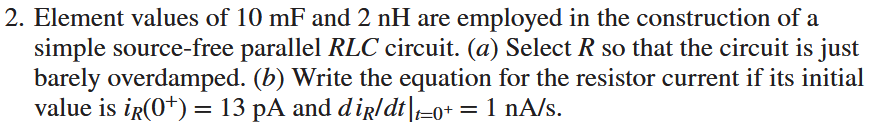
\includegraphics[width=0.8\textwidth]{9-2.png}
\end{center}
\begin{minipage}[t]{0.5\textwidth}
\vspace{0pt}
Given:
\begin{itemize}
    \item $C = 10$ mF
    \item $L = 2$ nH
\end{itemize}
\end{minipage}
\hfill
\begin{minipage}[t]{0.35\textwidth}
\vspace{0pt}
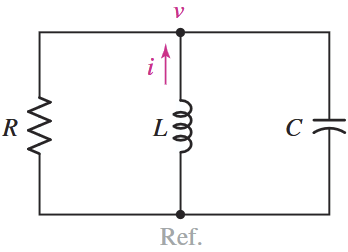
\includegraphics[width=\textwidth]{9-2-1.png}
\end{minipage}\\\\
\textbf{(a)} Find R such that the circuit is just barely overdamped.\\\\
For an overdamped circuit, $\alpha > \omega_0$. Substituting the values of $\alpha$ and $\omega_0$, we have:
\[\frac{1}{2RC}>\frac{1}{\sqrt{LC}}\]
\[\implies R < \frac{1}{2}\sqrt{\frac{L}{C}} = \frac{1}{2}\sqrt{\frac{[2\times10^{-9}\,\text{H}]}{[10\times10^{-3}\,\text{F}]}}=223.606\times10^{-6}\,\Omega\]
Thus, just barely less than $223.606\,\mu\Omega$,
\[\boxed{R=223.5\times10^{-6}\,\Omega}\]
\textbf{(b)} Find $i_R(t)$ given $i_R(0^+) = 13$ pA, and $di_R/dt(0^+) = 1$ nA/s.\\\\
Since the circuit is overdamped, the response is of the form:
\[i_R(t) = A_1e^{s_1t} + A_2e^{s_2t}\]
Where $s_1$ and $s_2$ are the roots of the characteristic equation:
\[s_{1,2}=-\alpha \pm \sqrt{\alpha^2 - \omega_0^2}\]
\[\alpha = \frac{1}{2RC} = \frac{1}{2[223.5 \times 10^{-6}\,\Omega] [10 \times 10^{-3}\,\text{F}]} = 223.71\times10^{3}\]
\[\omega_0 = \frac{1}{\sqrt{LC}} = \frac{1}{\sqrt{[2\times10^{-9}\,\text{H}][10\times10^{-3}\,\text{F}]}} = 223.6\times10^{3}\]
\[s_1 = -230.72\times10^{3},\quad s_2 = -216.69\times10^{3}\]
\newpage\noindent
Now solving for $A_1$ and $A_2$ using the initial conditions:
\begin{itemize}
    \item $i_R(0^+) = 13\times10^{-12}$ A
    \[i_R(0^+) = A_1 + A_2 = 13\times10^{-12}\]
    \item $\left.\frac{di_R}{dt}\right|_{t=0^+} = 1\times10^{-9}$ A/s
    \[ \frac{di_R}{dt}(0^+) = A_1s_1 + A_2s_2 = 1\times10^{-9} \]
\end{itemize}
Solving the system of equations, we have:
\[A_1 = 2.13\times10^{-10},\quad A_2 = -2.00\times10^{-10}\]
Thus, the time domain response is:
\[\boxed{i_R(t) = (2.13\times10^{-10})e^{-230.72\times10^{3}t} + (-2.00\times10^{-10})e^{-216.69\times10^{3}t}\,\text{A}}\]
\underline{Note:} We could also solve this using laplace transforms using the governing equation (KCL):
\[\frac{v}{R}+\left(i_0+\frac{1}{L}\int_0^t v(t')\,dt'\right)+C\frac{dv}{dt} = 0\]
\[\implies V(s)= \frac{RLCv_0s-RLi_0}{RLCs^2+Ls+R}\]
Finding the roots of the denominator gives us $s_1$ and $s_2$:
\[V(s) = v_0\left[\frac{s}{(s-s_1)(s-s_2)}\right]-\frac{i_0}{C}\left[\frac{1}{(s-s_1)(s-s_2)}\right]\]
Compare to form:
\[\frac{s}{(s+a)(s+b)}\rightarrow \frac{1}{b-a}(be^{-bt}-ae^{-at})\]
\[\frac{1}{(s+a)(s+b)}\rightarrow \frac{1}{b-a}(e^{-at}-e^{-bt})\]
Be careful with the lapace transform of the integral term. Since we already included the initial condition $i_0$, we can assume the integral has zero initial conditions when taking the laplace transform, so $\mathcal{L}\left\{\int_0^t v(t')\,dt'\right\} = \frac{V(s)}{s}$, not $\frac{V(s)}{s} + \text{initial conditions}$.

\section*{9.13}
\vspace{-2em}
\begin{center}
    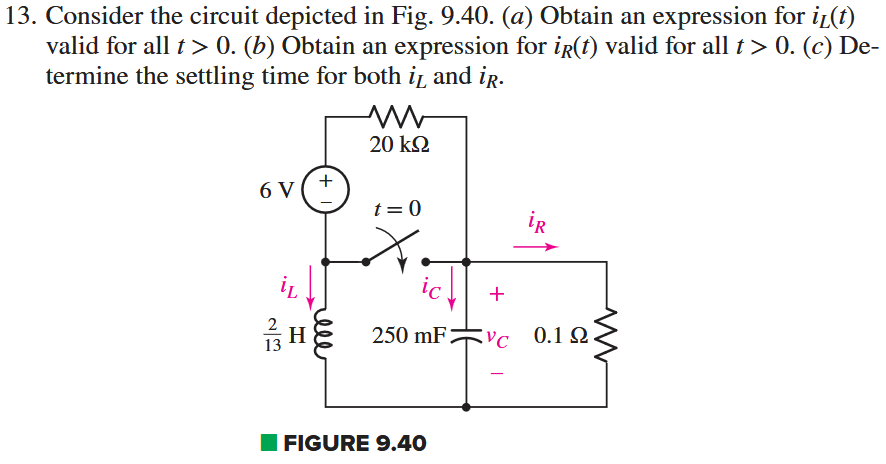
\includegraphics[width=0.8\textwidth]{9-13.png}
\end{center}
Initial conditions ($t<0$) at steady state: the capacitor is an open circuit and the inductor is a short circuit.
\begin{center}
    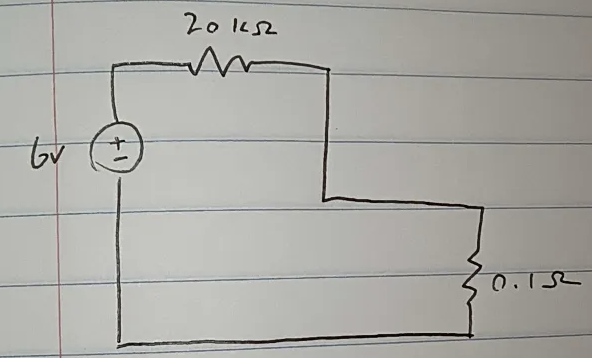
\includegraphics[width=0.4\textwidth]{9-13-1.png}
\end{center}
Using voltage division, we can find the voltage across the 0.1 $\Omega$ resistor (which is equal to $v_C$):
\[v_{0.1\Omega} = \frac{[0.1\,\Omega]}{[0.1 + 20\times10^3\,\Omega]} [6\,\text{V}]=29.99\times10^{-6},\text{V}\]
The current through the resistors is equal to $i_L$:
\[i=\frac{[6\,\text{V}]}{[0.1 + 20\times10^3\,\Omega]}=299.99\times10^{-6}\,\text{A}\]
Thus the initial conditions are:
\begin{itemize}
    \item $i_R(0^-) = i_L(0^-) = 299.99\times10^{-6}$ A, $i_C(0^-) = 0$ A
    \item $v_{0.1\Omega}(0^-) = v_C(0^-) = 29.99\times10^{-6}$ V, $v_L(0^-) = 0$ V
\end{itemize}
After the switch is closed, current from the 6V source will follow the path of least resistance, thus it will flow through the switch back to the source, and not through the rest of the circuit. We can therefore redraw the circuit for $t>0$ as a source free parallel RLC circuit.
\newpage\noindent
\textbf{(a)} Find $i_L(t)$ for $t>0$.\\\\
First, we determine if the circuit is overdamped, underdamped, or critically damped. We have:
\[\alpha = \frac{1}{2RC} = \frac{1}{2[0.1\,\Omega][250\times10^{-3}\,\text{F}]} = 20\]
\[\omega_0 = \frac{1}{\sqrt{LC}} = \frac{1}{\sqrt{[0.1538\,\text{H}][250\times10^{-3}\,\text{F}]}} = 5.099\]
Since $\alpha > \omega_0$, the circuit is overdamped, and the response is of the form:
\[i_L(t) = A_1e^{s_1t} + A_2e^{s_2t}\]
Where $s_1$ and $s_2$ are the roots of the characteristic equation:
\[s_{1,2}=-\alpha \pm \sqrt{\alpha^2 - \omega_0^2}\]
\[s_1 = -39.33,\quad s_2 = -0.66\]
Now solving for $A_1$ and $A_2$ using the initial conditions:
\begin{itemize}
    \item $i_L(0^+) = 299.99\times10^{-6}$ A
    \[i_L(0^+) = A_1 + A_2 = 299.99\times10^{-6}\]
    \item $v_L(0^+)=L\left.\frac{di_L}{dt}\right|_{t=0^+}=v_C(0^+)\implies\left.\frac{di_L}{dt}\right|_{t=0^+} = 194.93\times10^{-6}$ A/s
    \[ \left.\frac{di_L}{dt}\right|_{t=0^+} = A_1s_1 + A_2s_2 = 194.93\times10^{-6} \]
\end{itemize}
\underline{Note:} Although voltage across the capacitor can't change instantaneously, the current through the inductor can change instantaneously, thus when the switch closes, $v_L$ will jump from 0V to $v_C(0^+)$.\\\\
Solving the system of equations, we have:
\[A_1 = -1.02\times10^{-5},\quad A_2 = 3.10\times10^{-4}\]
Thus, the time domain response is:
\[\boxed{i_L(t) = (-1.02\times10^{-5})e^{-39.33t} + (3.10\times10^{-4})e^{-0.66t}\,\text{A}}\]
\textbf{(b)} Find $i_R(t)$ for $t>0$.\\\\
We can first find $v_R(t)=v_C(t)$ since they are in parallel, and then use Ohm's law to find $i_R(t)$. Since we know that the circuit is overdamped, the form of the response is the same as $i_L(t)$, so we can write:
\[V_C(t) = B_1e^{s_1t} + B_2e^{s_2t}\]
Where $s_1$ and $s_2$ are the same as before. Now solving for $B_1$ and $B_2$ using the initial conditions:
\begin{itemize}
    \item $v_C(0^+) = 29.99\times10^{-6}$ V
    \[ v_C(0^+) = B_1 + B_2 = 29.99\times10^{-6} \]
    \item $ \left.\frac{dv_C}{dt}\right|_{t=0^+} $:\\\\
    Using KCL at the top node, we have:
    \[i_R(0^+) + i_L(0^+) + i_C(0^+) = 0\implies i_C(0^+) = -\frac{v}{R}-[299.99\times10^{-6}\,\text{A}] = -599.98\times10^{-6}\,\text{A}\]
    \[i_C(0^+) = C\left.\frac{dv_C}{dt}\right|_{t=0^+}\implies \left.\frac{dv_C}{dt}\right|_{t=0^+} = -23.99\times10^{-4}\,\text{V/s}\]
\end{itemize}
Solving the system of equations, we have:
\[B_1 = 6.15\times10^{-5},\quad B_2 = -3.15\times10^{-5}\]
Thus, the time domain response for $i_R(t) = \frac{1}{R}V_C(t)$ is:
\[\boxed{i_R(t)=\frac{1}{0.1}\left(6.15\times10^{-5}e^{-39.33t} - 3.15\times10^{-5}e^{-0.66t}\right)\,\text{A}}\]
\textbf{(c)} Find the settling time for $i_L(t)$ and $i_R(t)$.\\\\
\textbf{Settling time} is the time it takes for the response to decay and remain below 1\% of its maximum value $|i_m|$.\\\\
For an overdamped response, we can neglect the faster root and look at the slower root (the one closer to zero):
\[i_L(t)\approx 3.1\times10^{-4}e^{-0.66t}\implies i_L(t_s) = 0.01\cdot3.1\times10^{-4}=3.1\times10^{-4}e^{-0.66t_s}\]
\[\implies \boxed{t_s = 6.97\,\text{s}\quad (\text{for }i_L(t))}\]
Similarly, for $i_R(t)$, we have:
\[i_R(t)\approx \frac{1}{0.1}\left(-3.15\times10^{-5}e^{-0.66t}\right)\implies i_R(t_s) = 0.01\cdot\frac{1}{0.1}\left|-3.15\times10^{-5}\right|=\frac{1}{0.1}\left|-3.15\times10^{-5}e^{-0.66t_s}\right|\]
\[\implies \boxed{t_s = 6.97\,\text{s}\quad (\text{for }i_R(t))}\]
Since they share the same root, they have the same settling time.

\section*{9.16}
\vspace{-2em}
\begin{center}
    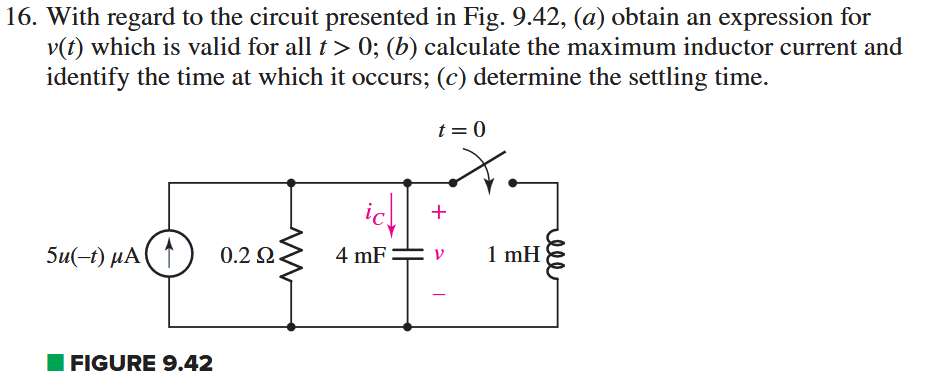
\includegraphics[width=0.8\textwidth]{9-16.png}
\end{center}
Notice that the current source is $5u(-t)$ which means that the current source is only on for $t<0$, and turns off at $t=0$!\\\\
For $t<0$, at steady state (capacitor is an open circuit, inductor is disconnected):
\begin{itemize}
    \item $i_L(0^-) = 0$ A, $v_L(0^-) = 0$ V
    \item $i_R(0^-) = 5\,\mu$A, $v_R(0^-) = [5\,\mu\text{A}][0.2\,\Omega] = 1\times10^{-6}$ V
    \item $i_C(0^-) = 0$ A, $v_C(0^-) = 1\times10^{-6}$ V
\end{itemize}
For $t>0$, the current source turns off, and the inductor is now connected. Since the capacitor voltage doesn't change instantaneously:
\begin{itemize}
    \item $v_R(0^+) = v_C(0^+) = v_L(0^+) = 1\times10^{-6}$ V
    \item $i_R(0^+) = 5\,\mu$A
    \item Since the inductor current cannot change instantaneously, $i_L(0^+) = i_L(0^-) = 0$ A
    \item $\left.\frac{dv}{dt}\right|_{t=0^+} = \frac{1}{C}i_C(0^+)$:
    Using KCL at the top node, we have:
    \[i_R(0^+) + i_L(0^+) + i_C(0^+) = 0 \implies i_C(0^+) = -i_R(0^+)= -5\,\mu\text{A}\]
    \[\implies \left.\frac{dv}{dt}\right|_{t=0^+} = \frac{[-5\times10^{-6}\,\text{A}]}{[4\times10^{-3}\,\text{F}]} = -0.00125\,\text{V/s}\]
\end{itemize}
\textbf{(a)} Find $v(t)$ for $t>0$.\\\\
First, we determine if the circuit is overdamped, underdamped, or critically damped. We have:
\[\alpha = \frac{1}{2RC} = \frac{1}{2[0.2\,\Omega][4\times10^{-3}\,\text{F}]} = 625\]
\[\omega_0 = \frac{1}{\sqrt{LC}} = \frac{1}{\sqrt{[10^{-3}\,\text{H}][4\times10^{-3}\,\text{F}]}} = 500\]
Since $\alpha > \omega_0$, the circuit is overdamped, and the response is of the form:
\[v(t) = A_1e^{s_1t} + A_2e^{s_2t}\]
where $s_1$ and $s_2$ are the roots of the characteristic equation.
\[s_{1,2}=-\alpha \pm \sqrt{\alpha^2 - \omega_0^2}\]
\[s_1 = -1000,\quad s_2 = -250\]
Now solving for $A_1$ and $A_2$ using the initial conditions (using $v_C$ since everything is in parallel):
\begin{itemize}
    \item $v_C(0^+) = 1\times10^{-6}$ V
    \[v_C(0^+) = A_1 + A_2 = 1\times10^{-6}\]
    \item $\left.\frac{dv_C}{dt}\right|_{t=0^+} = -0.00125$ V/s
    \[ \left.\frac{dv_C}{dt}\right|_{t=0^+} = A_1s_1 + A_2s_2 = -0.00125 \]
\end{itemize}
Solving the system of equations, we have:
\[A_1 = 1.33\times10^{-6},\quad A_2 = -3.33\times10^{-7}\]
Thus, the time domain response is:
\[\boxed{v(t) = (1.33\times10^{-6})e^{-1000t} + (-3.33\times10^{-7})e^{-250t}\,\text{V}}\]
\textbf{(b)} Find the max inductor current and the time at which it occurs.\\\\
The inductor current is given by
\[i_L(t)=i_L(0^+) + \int_0^t \frac{v_L(t')}{L} dt'\]
Since $i_L(0^+) = 0$ A and $v_L(t) = v(t)$, we have:
\[i_L(t)= \frac{1}{10^{-3}}\int_0^t ((1.33\times10^{-6})e^{-1000t'} + (-3.33\times10^{-7})e^{-250t'})\,dt'\]
\[i_L(t)= 1.33\times10^{-6}(e^{-250t}-e^{-1000t})\]
The current is maximum when $\frac{di_L}{dt} = 0$:
\[\frac{di_L}{dt} = 1.33\times10^{-6}(-250e^{-250t}+1000e^{-1000t})=0\implies \boxed{t=1.848\times10^{-3}\,\text{s}}\]
Substituting back into $i_L(t)$, we have:
\[\boxed{i_L(1.848\times10^{-3}\,\text{s}) = 0.628\times10^{-6}\,\text{A}}\]
\textbf{(c)} Settling time for $v(t)$.\\\\
\[v(t)\approx -3.33\times10^{-7}e^{-250t}\implies v(t_s) = 0.01\cdot|-3.33\times10^{-7}|=|-3.33\times10^{-7}e^{-250t_s}|\]
\[\implies \boxed{t_s = 0.0184\,\text{s}}\]

\section*{9.21}
\vspace{-2em}
\begin{center}
    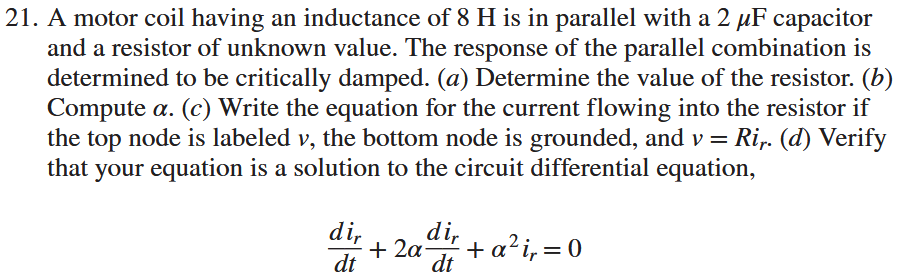
\includegraphics[width=0.8\textwidth]{9-21.png}
\end{center}
\textbf{(a)} For a critically damped parallel RLC circuit, we have $\alpha = \omega_0$.
\[\implies \frac{1}{2RC} = \frac{1}{\sqrt{LC}}\]
\[R= \frac{1}{2}\sqrt{\frac{L}{C}} = \frac{1}{2}\sqrt{\frac{[8\,\text{H}]}{[2\times10^{-6}\,\text{F}]}} = \boxed{1000\,\Omega}\]
\textbf{(b)} Find $\alpha$
\[\alpha = \frac{1}{2RC} = \frac{1}{2[1000\,\Omega][2\times10^{-6}\,\text{F}]} = \boxed{250\,\text{rad/s}}\]
\textbf{(c)} Find $i_R$:\\\\
Since the circuit is critically damped, the response is of the form:
\[v(t) = e^{-\alpha t}(A_1t + A_2)\]
Where $\alpha$ is the same as before.\\\\
\textbf{(d)} Show that it is a solution to the differential equation:
\[ \frac{d^2i_R}{dt^2} + 2\alpha \frac{di_R}{dt} + \alpha^2 i_R = 0 \]
Find derivatives:
\begin{align*}
\frac{di_R}{dt} &= A_1 e^{-\alpha t} - \alpha(A_1 t + A_2)e^{-\alpha t} \\
&= e^{-\alpha t} \left[ A_1 - \alpha(A_1 t + A_2) \right]
\end{align*}
\begin{align*}
\frac{d^2i_R}{dt^2} &= -\alpha e^{-\alpha t} \left[ A_1 - \alpha(A_1 t + A_2) \right] + e^{-\alpha t} [-\alpha A_1] \\
&= e^{-\alpha t} \left[ -\alpha A_1 + \alpha^2(A_1 t + A_2) - \alpha A_1 \right] \\
&= e^{-\alpha t} \left[ -2\alpha A_1 + \alpha^2(A_1 t + A_2) \right]
\end{align*}
Plugging these results back into the original equation:
\begin{align*}
\text{LHS} &= e^{-\alpha t} \left[ -2\alpha A_1 + \alpha^2(A_1 t + A_2) \right] + 2\alpha e^{-\alpha t} \left[ A_1 - \alpha(A_1 t + A_2) \right] + \alpha^2 e^{-\alpha t} (A_1 t + A_2) \\
&= e^{-\alpha t} \Big[ -2\alpha A_1 + \alpha^2(A_1 t + A_2) + 2\alpha A_1 - 2\alpha^2(A_1 t + A_2) + \alpha^2(A_1 t + A_2) \Big] \\
&= e^{-\alpha t} \Big[ (-2\alpha A_1 + 2\alpha A_1) + (\alpha^2 - 2\alpha^2 + \alpha^2)(A_1 t + A_2) \Big] \\
&= e^{-\alpha t} [0 + 0] = 0
\end{align*}

\section*{9.26}
\vspace{-2em}
\begin{center}
    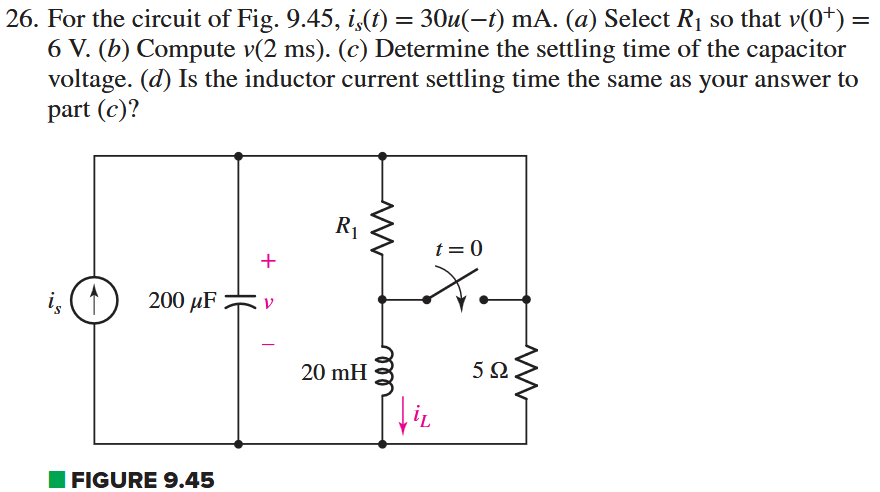
\includegraphics[width=0.8\textwidth]{9-26.png}
\end{center}
\textbf{(a)} Find $R_1$ such that $v(0^+) = 6$ V.\\\\
For $t<0$ at steady state, the capacitor is an open circuit and the inductor is a short circuit and $i_s = 30$ mA. 
\begin{center}
    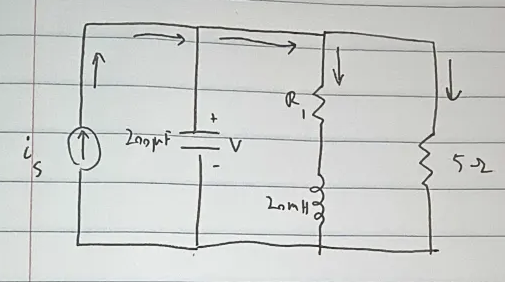
\includegraphics[width=0.4\textwidth]{9-26-1.png}
\end{center}
Thus, 
\[R_{eq} = \frac{R_1\cdot[5\,\Omega]}{R_1+[5\,\Omega]}\]
\[v(0^-) = i_s \cdot R_{eq} = [30\times10^{-3}\,\text{A}] \cdot \frac{R_1\cdot[5\,\Omega]}{R_1+[5\,\Omega]}=6\,\text{V}\]
\[\implies \frac{R_1\cdot[5\,\Omega]}{R_1+[5\,\Omega]} = 200\]
However, this is physically impossible. Looking at the circuit for $t>0$:
\begin{center}
    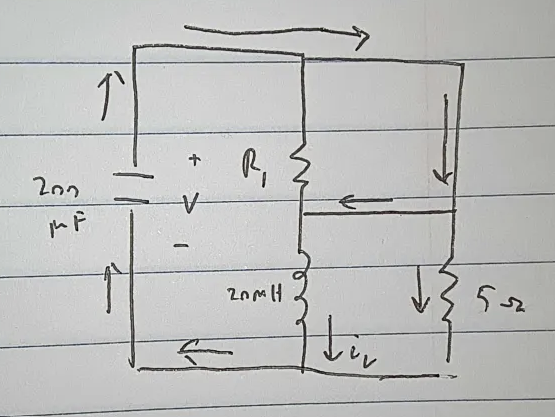
\includegraphics[width=0.4\textwidth]{9-26-2.png}
\end{center}
Since the inductor maintains current in the same direction, the switch actually shorts $R_1$. Thus, it makes sense that we can't find a value of $R_1$ that satisfies the condition, since $R_1$ is effectively removed from the circuit for $t>0$.\\\\
\textbf{(b)} Find $v(2\,\text{ms})$.\\\\
Without $R_1$, this is just a source free parallel RLC circuit. First we determine if the circuit is overdamped, underdamped, or critically damped. We have:
\[\alpha = \frac{1}{2RC} = \frac{1}{2[5\,\Omega][200\times10^{-6}\,\text{F}]} = 500\]
\[\omega_0 = \frac{1}{\sqrt{LC}} = \frac{1}{\sqrt{[20\times10^{-3}\,\text{H}][200\times10^{-6}\,\text{F}]}} = 500\]
Since $\alpha = \omega_0$, the circuit is critically damped, and the response is of the form:
\[v(t) = e^{-\alpha t}(A_1t + A_2)\]
Now finding the initial conditions:
\begin{itemize}
    \item Assuming that $v(0^+) = 6$ V
    \item $\left.\frac{dv}{dt}\right|_{t=0^+} = \frac{1}{C}i_C(0^+)$:\\\\
    Using KCL at the top node, we have:
\[i_R(0^+) + i_L(0^+) + i_C(0^+) = 0\implies i_C(0^+) = -\frac{v}{R}-i_L(0^+) =-\frac{[6\,\text{V}]}{[5\,\Omega]} - [30\times10^{-3}\,\text{A}]=-1.23\,\text{A}\]
Since the inductor current cannot change instantaneously, $i_L(0^+) = i_L(0^-) = 30$ mA. Thus,
\[\implies \left.\frac{dv}{dt}\right|_{t=0^+} = \frac{[-1.23\,\text{A}]}{[200\times10^{-6}\,\text{F}]} = -6150\,\text{V/s}\]
\end{itemize}
Solving for $A_1$ and $A_2$:
\begin{itemize}
    \item $v(0^+) = 6$ V
    \[v(0^+) = A_2 = 6\,\text{V}\]
    \item $\left.\frac{dv}{dt}\right|_{t=0^+} = -6150$ V/s
    \[ \left.\frac{dv}{dt}\right|_{t=0^+} = A_1 - \alpha A_2 = -6150 \]
\end{itemize}
\[\implies A_1 = -3150,\quad A_2 = 6\]
Thus, the time domain response is:
\[\boxed{v(t) = e^{-500t}(-3150t + 6)\,\text{V}}\]
\[\implies \boxed{v(2\,\text{ms}) = -0.110\,\text{V}}\]
\textbf{(c)} Find the settling time of the capacitor voltage.\\\\
Since the circuit is critically damped, we can't just neglect a root. Thus we would need a numerical solver instead.\\\\
We find that
\[v_m=-0.894\,\text{V}\]
\[\boxed{t_s = 0.01718\,\text{s}}\]
\textbf{(d)} Is the inductor current settling time the same?\\\\
Yes, since the inductor current has the same form of response as the capacitor voltage, they will have the same settling time.

\section*{9.30}
\vspace{-2em}
\begin{center}
    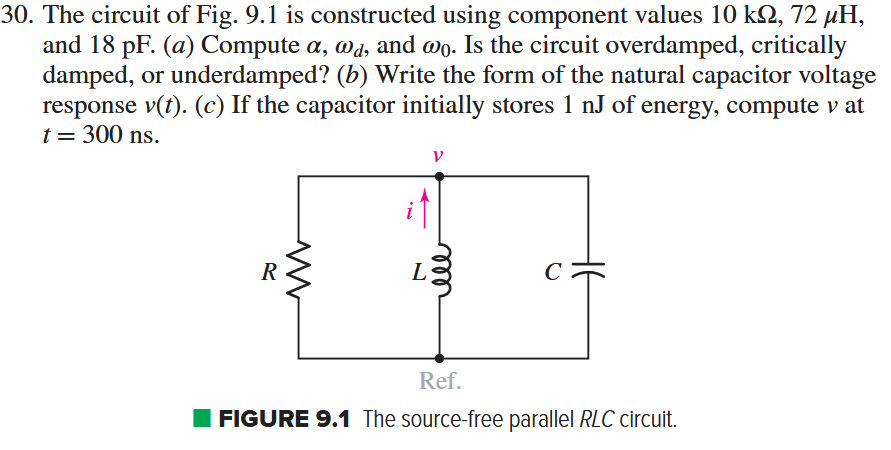
\includegraphics[width=0.8\textwidth]{9-30.png}
\end{center}
\textbf{(a)} Find $\alpha$, $\omega_0$, and $\omega_d$. First we determine if the circuit is overdamped, underdamped, or critically damped. We have:
\[\alpha = \frac{1}{2RC} = \frac{1}{2[10\times10^3\,\Omega][18\times10^{-12}\,\text{F}]} = \boxed{2.777\times10^6 \,\text{rad/s}}\]
\[\omega_0 = \frac{1}{\sqrt{LC}} = \frac{1}{\sqrt{[72\times10^{-6}\,\text{H}][18\times10^{-12}\,\text{F}]}} = \boxed{27.777\times10^6 \,\text{rad/s}}\]
Since $\alpha < \omega_0$, the circuit is underdamped, and the damped natural frequency is given by:
\[\omega_d = \sqrt{\omega_0^2 - \alpha^2} = \sqrt{(27.777\times10^6)^2 - (2.777\times10^6)^2} = \boxed{27.631\times10^6 \,\text{rad/s}}\]
\textbf{(b)} The form of the response for $v(t)$ is:
\[\boxed{v(t) = e^{-\alpha t}(B_1 \cos \omega_d t + B_2 \sin \omega_d t)}\]
\textbf{(c)} Find $v(300\,\text{ns})$.\\\\
Given that the capacitor stores 1 nJ of energy at $t=0$, we can find the initial voltage across the capacitor:
\[w = \frac{1}{2}Cv^2\implies v(0^+) = \sqrt{\frac{2w}{C}} = \sqrt{\frac{2[1\times10^{-9}\,\text{J}]}{[18\times10^{-12}\,\text{F}]}} = 10.54\,\text{V}\]
Assuming there is zero current through the inductor at $t=0^+$, we can find $dv/dt$ at $t=0^+$ using KCL at the top node:
\[i_R(0^+) + i_L(0^+) + i_C(0^+) = 0 \implies i_C(0^+) = -\frac{v(0^+)}{R} \]
\[i_C(0^+) = 0.00105\,\text{A} \implies \left.\frac{dv}{dt}\right|_{t=0^+} = \frac{i_C(0^+)}{C} = \frac{[0.00105\,\text{A}]}{[18\times10^{-12}\,\text{F}]} = 58.55\times10^6\,\text{V/s}\]
Now solving for $B_1$ and $B_2$:
\begin{itemize}
    \item $v(0^+) = 10.54$ V
    \[v(0^+) = B_1 = 10.54\,\text{V}\]
    \item $\left.\frac{dv}{dt}\right|_{t=0^+} = 58.55\times10^6$ V/s
    \[ \left.\frac{dv}{dt}\right|_{t=0^+} = -\alpha B_1 + \omega_d B_2 = 58.55\times10^6 \]
\end{itemize}
Solving for $B_1$ and $B_2$, we have:
\[B_1 = 10.54,\quad B_2 = 3.175\]
Thus, the time domain response is:
\[\boxed{v(t) = e^{-2.777\times10^6 t}(10.54 \cos (27.631\times10^6 t) + 3.175 \sin (27.631\times10^6 t))\,\text{V}}\]
\[\implies \boxed{v(300\,\text{ns}) = -0.682,\text{V}}\]

\section*{9.35}
\vspace{-2em}
\begin{center}
    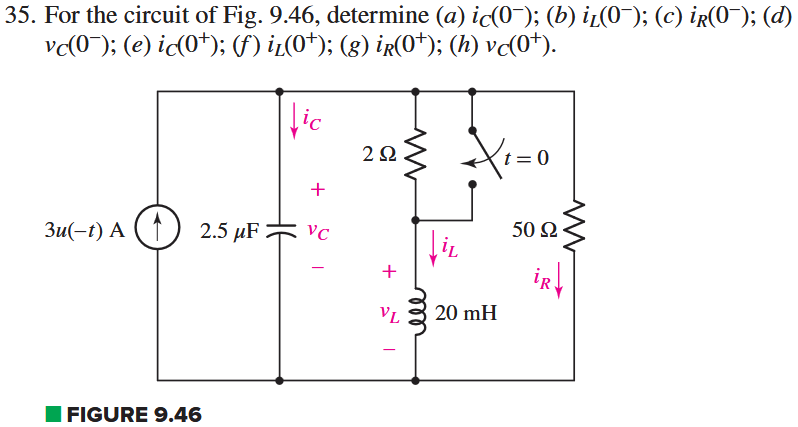
\includegraphics[width=0.8\textwidth]{9-35.png}
\end{center}
Circuit for $t<0$:
\begin{center}
    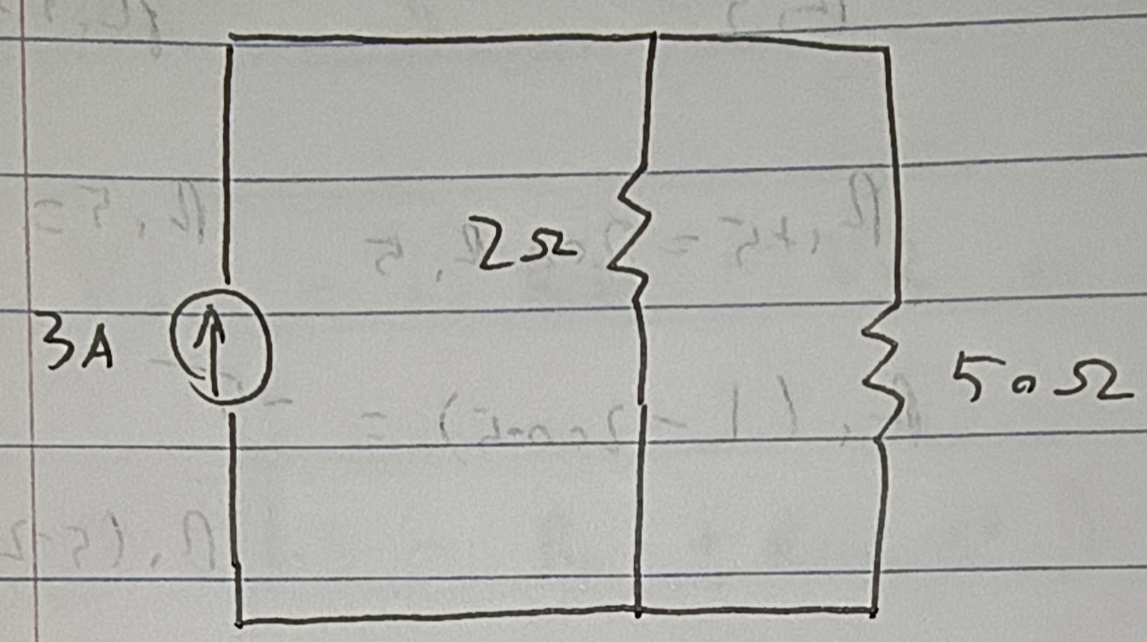
\includegraphics[width=0.4\textwidth]{9-35-1.png}
\end{center}
Voltage across each parallel branch is then:
\[R_{eq} = \frac{[2\,\Omega]\cdot[50\,\Omega]}{[2+50\,\Omega]} = 1.92\,\Omega\]
\[V = [3\,\text{A}][1.92\,\Omega] = 5.76\,\text{V}\]
Current division for each branch:
\[i_{2\Omega} = \frac{\frac{1}{[2\,\Omega]}}{\frac{1}{[1.92\,\Omega]}}[3\,\text{A}] = 2.88\,\text{A}\]
\[i_{50\Omega} = \frac{\frac{1}{[50\,\Omega]}}{\frac{1}{[1.92\,\Omega]}}[3\,\text{A}] = 0.115\,\text{A}\]
Therefore:
\[
\fbox{
\parbox{0.5\textwidth}{
\begin{itemize}
    \item $i_C(0^-) = 0$ A
    \item $i_L(0^-) = 2.88$ A
    \item $i_R(0^-) = 0.115$ A
    \item $v_C(0^-) = v_L(0^-) = v_R(0^-) = 5.76$ V
\end{itemize}
}
}
\]
Circuit for $t>0$:
\begin{center}
    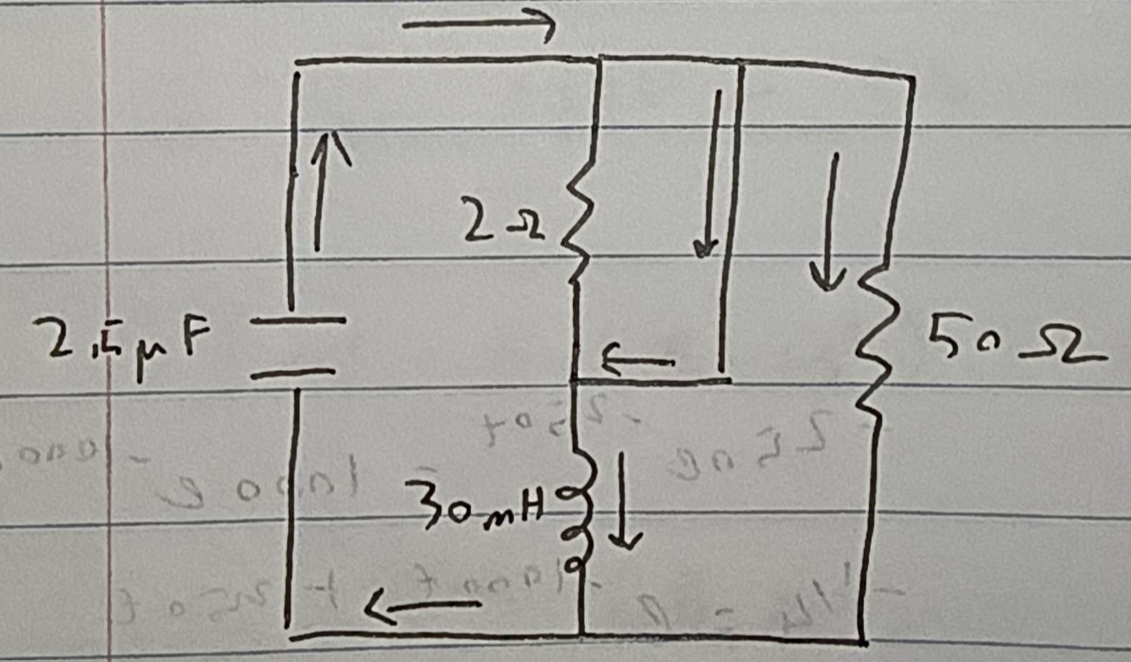
\includegraphics[width=0.4\textwidth]{9-35-2.png}
\end{center}
Voltage across capacitors don't change instantaneously, and current through inductors don't change instantaneously. Thus:
\[i_R(0^+) = \frac{v(0^+)}{R} = \frac{[5.76\,\text{V}]}{[50\,\Omega]} = 0.115\,\text{A}\]
By KCL at the top node:
\[i_R(0^+) + i_L(0^+) + i_C(0^+) = 0\implies i_C(0^+) = -i_R(0^+) - i_L(0^+) = -[0.115\,\text{A}] - [2.88\,\text{A}] = -2.995\,\text{A}\]
Thus, the initial conditions for $t>0$ are:
\[
\fbox{
\parbox{0.5\textwidth}{
\begin{itemize}
    \item $i_C(0^+) = -2.995$ A
    \item $i_L(0^+) = 2.88$ A
    \item $i_R(0^+) = 0.115$ A
    \item $v_C(0^+) = v_L(0^+) = v_R(0^+) = 5.76$ V
\end{itemize}
}
}
\]

\section*{9.46}
\vspace{-2em}
\begin{center}
    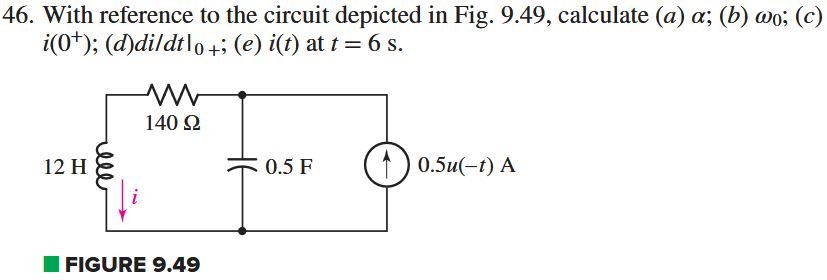
\includegraphics[width=0.8\textwidth]{9-46.png}
\end{center}
\textbf{(a)} Find $\alpha$. (Series RLC circuit)
\[\alpha = \frac{R}{2L}=\frac{[140\,\Omega]}{2[12\,\text{H}]} = \boxed{5.833\,\text{rad/s}}\]
\textbf{(b)} Find $\omega_0$.
\[\omega_0 = \frac{1}{\sqrt{LC}} = \frac{1}{\sqrt{[12\,\text{H}][0.5\,\text{F}]}} = \boxed{0.408\,\text{rad/s}}\]
Since $\alpha>\omega_0$, this circuit is overdamped.\\\\
\textbf{(c)} Find $i(0^+)$.\\\\
For $t<0$ at steady state, the current through the inductor is equal to the source and since the inductor current cannot change instantaneously, we have:
\[\boxed{i(0^+) = i(0^-) = 0.5\,\text{A}}\]
\textbf{(d)} Find $di/dt$ at $t=0^+$.\\\\
Using the voltage over the inductor we can find $di/dt$ at $t=0^+$:
\[v_L(0^+) = L \left.\frac{di}{dt}\right|_{t=0^+}\]
At steady state at $t=0^-$ the voltage drop across the resistor is equal to the voltage across the capacitor (they are in parallel), and since the voltage across the capacitor can't change instantaneously, we have:
\[v_C(0^-) = v_C(0^+) = v_R(0^-) = [140\,\Omega][0.5\,\text{A}] = 70\,\text{V}\]
Thus, subtracting the voltage drop across the resistor at $t=0^+$ from the voltage across the capacitor, we can find the voltage across the inductor at $t=0^+$:
\[v_L(0^+) = v_C(0^+) - v_R(0^+) = [70\,\text{V}] - [140\,\Omega][0.5\,\text{A}] = 0\,\text{A}\]
\[\implies \boxed{\left.\frac{di}{dt}\right|_{t=0^+} = 0\,\text{A/s}}\]
\textbf{(e)} Find $i(6)$.\\\\
Since the circuit is overdamped, the response is of the form:
\[i(t) = A_1e^{s_1t} + A_2e^{s_2t}\]
Where $s_1$ and $s_2$ are the roots of the characteristic equation:
\[s_{1,2}=-\alpha \pm \sqrt{\alpha^2 - \omega_0^2}\]
\[s_1 = -11.65,\quad s_2 = -0.0142\]
Now solving for $A_1$ and $A_2$ using the initial conditions:
\begin{itemize}
    \item $i(0^+) = 0.5$ A
    \[i(0^+) = A_1 + A_2 = 0.5\]
    \item $\left.\frac{di}{dt}\right|_{t=0^+} = 0$ A/s
    \[ \left.\frac{di}{dt}\right|_{t=0^+} = A_1s_1 + A_2s_2 = 0 \]
\end{itemize}
Solving the system of equations, we have:
\[A_1 = -6.1\times10^{-4},\quad A_2 = 0.501\]
Thus, the time domain response is:
\[\boxed{i(t) = (-6.1\times10^{-4})e^{-11.65t} + (0.501)e^{-0.0142t}\,\text{A}}\]
\[\implies \boxed{i(6) = 0.46\,\text{A}}\]

\section*{9.50}
\vspace{-2em}
\begin{center}
    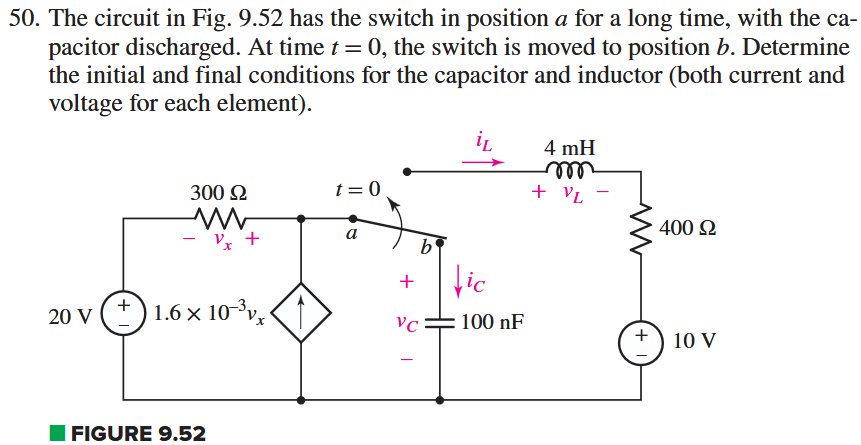
\includegraphics[width=0.8\textwidth]{9-50.png}
\end{center}
\underline{Note:} This diagram is confusing so I'm going to be using my own interpretation of the circuit.\\\\
Circuit for $t<0$:
\begin{center}
    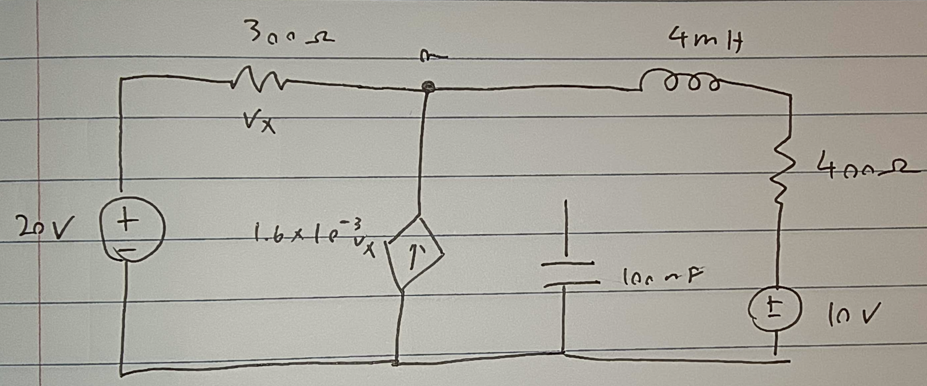
\includegraphics[width=0.6\textwidth]{9-50-2.png}
\end{center}
Given that the capacitor is \textit{discharged}, the voltage across the capacitor is 0V at $t=0^-$. At steady state, the capacitor is also an open circuit, so there is no current.\\\\
KCL at the top node gives us:
\[v_x = v_a-20\]
\[\frac{v_a-20}{[300\,\Omega]}-1.6\times10^{-3}(v_a-20) +\frac{v_a-10}{[400\,\Omega]}= 0\]
\[\implies v_a = 14.094\,\text{V}\]
Thus, the current going through the 400 $\Omega$ resistor is:
\[i = \frac{v_a-10}{[400\,\Omega]} = 0.0102\,\text{A}\]
Since the inductor is a short circuit in series with the 400 $\Omega$ resistor, the current through the inductor is also 0.0102 A. Thus, the initial conditions for $t<0$ are:
\begin{itemize}
    \item $i_L(0^-) = 0.0102$ A, $v_L(0^-) = 0$ V
    \item $i_C(0^-) = 0$ A, $v_C(0^-) = 0$ V
\end{itemize}
Circuit for $t>0$:
\begin{center}
    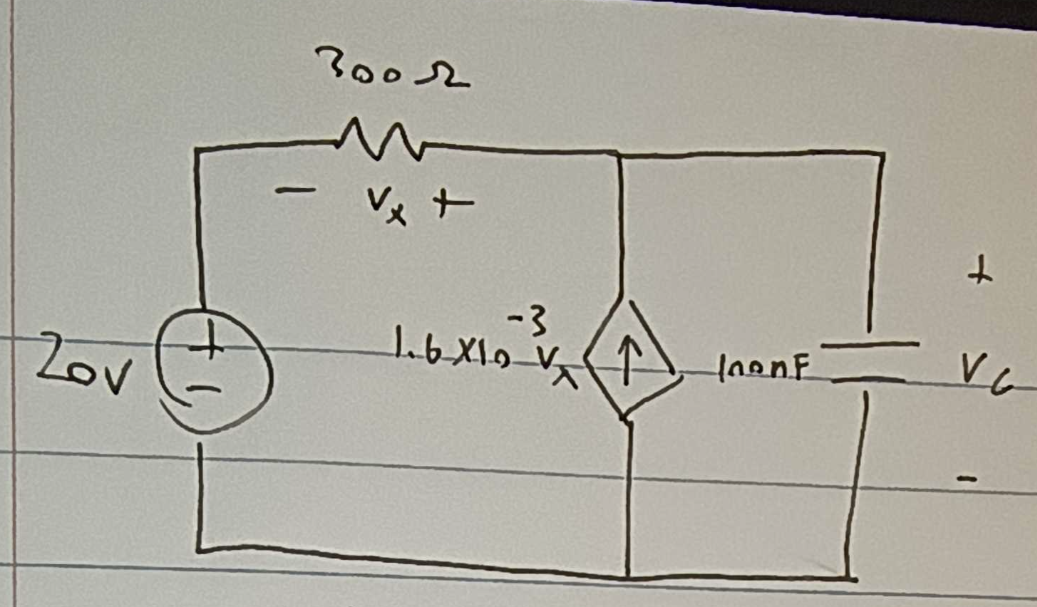
\includegraphics[width=0.5\textwidth]{9-50-1.png}
\end{center}
At steady state, the inductor is completely cut off, so it has zero current and voltage. The capacitor is an open circuit with zero current, but we can find its voltage.\\\\
Using KCl at the top node:
\[\frac{v_a-20}{[300\,\Omega]}-1.6\times10^{-3}(v_a-20) = 0\]
\[\implies v_a = 20\,\text{V}\]
Thus, the voltage across the capacitor is also $v_a=20$ V.
\begin{itemize}
    \item $i_L(0^+) = 0$ A, $v_L(0^+) = 0$ V
    \item $i_C(0^+) = 0$ A, $v_C(0^+) = 20$ V
\end{itemize}

\section*{9.54}
\vspace{-2em}
\begin{center}
    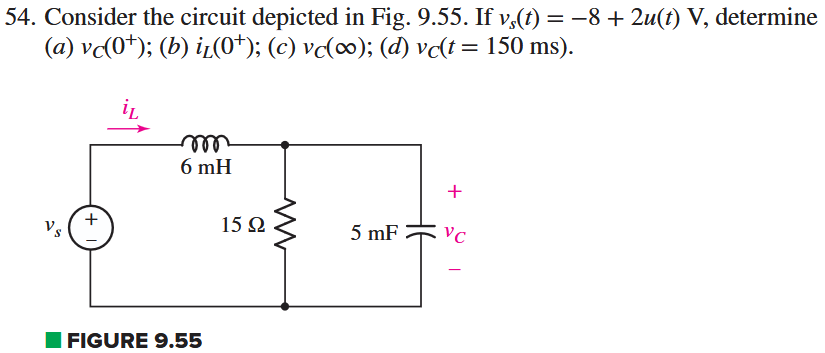
\includegraphics[width=0.8\textwidth]{9-54.png}
\end{center}
The voltage source has 2 states:
\begin{itemize}
    \item $v_s = -8$ V for $t<0$
    \item $v_s = -6$ V for $t>0$
\end{itemize}
\textbf{(a)} Find $v_C(0^+)$.\\\\
For $t<0$, at steady state:
\[v_s = v_C(0^-) = -8\,\text{V}\]
Since the voltage across the capacitor cannot change instantaneously, we have:
\[\boxed{v_C(0^+) = v_C(0^-) = -8\,\text{V}}\]
\textbf{(b)} Find $i_L(0^+)$.\\\\
Since the inductor current cannot change instantaneously, we can use $i_L(0^-)$. Since the inductor is in series with the 15 $\Omega$ resistor, we can find the current through the inductor at $t=0^-$ using Ohm's law:
\[i_L(0^-) = \frac{v_s}{R} = \frac{[-8\,\text{V}]}{[15\,\Omega]} = -0.533\,\text{A}\]
\[\boxed{i_L(0^+) = i_L(0^-) = -0.533\,\text{A}}\]
\textbf{(c)} Find $v_C(\infty)$.\\\\
Same steps but with new value of $v_s$:
\[\boxed{v_s = v_C(\infty) = -6\,\text{V}}\]
\newpage\noindent
\textbf{(d)} Find $v_C(150\,\text{ms})$.\\\\
\underline{Solving for the FREE response:}\\
First, we determine if the circuit is overdamped, underdamped, or critically damped. Without the voltage source, it would be a parallel RLC circuit:
\[\alpha = \frac{1}{2RC} = \frac{1}{2[15\,\Omega][5\times10^{-3}\,\text{F}]} = 6.66\,\text{rad/s}\]
\[\omega_0 = \frac{1}{\sqrt{LC}} = \frac{1}{\sqrt{[6\times10^{-3}\,\text{H}][5\times10^{-3}\,\text{F}]}} = 182.57\,\text{rad/s}\]
Since $\alpha < \omega_0$, the circuit is underdamped, and the response is of the form:
\[v_C(t) = e^{-\alpha t}(B_1 \cos \omega_d t + B_2 \sin \omega_d t) + v_C(\infty)\]
Where $\omega_d = \sqrt{\omega_0^2 - \alpha^2} = 182.45\,\text{rad/s}$.\\\\
Finding initial conditions:
\[v_C(0^+) = v_C(0^-) = -8\,\text{V}\]
Using KCL at the top node:
\[i_L(0^+) + i_R(0^+) + i_C(0^+) = 0 \implies i_C(0^+) = -i_L(0^+) - i_R(0^+)\]
\[i_C(0^+) = -[-0.533\,\text{A}] - [-0.533\,\text{A}] = 1.066\,\text{A}\]
\[\implies \frac{dv_C}{dt}(0^+) = \frac{i_C(0^+)}{C} = \frac{[1.066\,\text{A}]}{[5\times10^{-3}\,\text{F}]} = 213.2\,\text{V/s}\]
Now solving for $B_1$ and $B_2$:
\begin{itemize}
    \item $v_C(0^+) = -8$ V
    \[v_C(0^+) = B_1 = -8 \]
    \item $\left.\frac{dv_C}{dt}\right|_{t=0^+} = 213.2$ V/s
    \[ \left.\frac{dv_C}{dt}\right|_{t=0^+} = -\alpha B_1 + \omega_d B_2 = 213.2 \]
\end{itemize}
\[\implies B_1 = -8, \quad B_2 = 0.876\]
Thus, the FREE response is:
\[v_{C,0}(t) = e^{-6.66 t}(-8 \cos (182.45 t) + 0.876 \sin (182.45 t))\]
\underline{Finding the TOTAL response}\\
The total response is the sum of the free response and the forced response (steady state value $v_C(\infty)$):
\[\boxed{v_C(t) = e^{-6.66 t}(-8 \cos (182.45 t) + 0.876 \sin (182.45 t)) - 6\,\text{V}}\]
\[\implies \boxed{v_C(150\,\text{ms}) = -3.93\,\text{V}}\]
\underline{Check this solution}
\end{document}